% Provenance (never printed): see sources/outline_sources.md (Year 1: litho-, bio- and
% chronostratigraphy; boundary stratotypes; mass extinctions as global markers; the
% international chart). Exercise and problem values in the Book 3 scratch calculator
% calc/ch24.py; the chart from figdata/bachelor-1/ics_chart.py (shared ics rows).
% The principles of relative dating, eras and periods are Book 1's (g7 geological-time) and
% are re-founded here. Mass extinctions belong to the biology series (recalled in prose);
% their Earth causes are the Year 2 volume's (phanerozoic-earth). Correlation of logs and
% unconformities are ch. 5's; facies ch. 21's; compaction ch. 23's. Radiometric dating is
% ch. 25's. Sequence stratigraphy, facies models and Walther's law are the Year 3 volume's;
% magnetostratigraphy too: prose pointers only. "Transgression" is explained in prose.
\chapter{The Stratigraphic Scale}\label{ch:b1:stratigraphic-scale}

On the beach of Itzurun, at Zumaia on the Basque coast, the cliffs are made of
thin beds of limestone and marl, tilted and repeated for hundreds of metres. At one
contact, where a pale limestone bed ends and red marls begin, a bronze disc
stamped with four letters is set into the rock (figure below). It is a golden
spike. It fixes, for the whole planet, the instant at which one division of
geological time --- the Selandian \omterm{def:b1:stratigraphic-scale:chronostratigraphy}{Stage} --- begins. A rock in Patagonia or in
Siberia is Selandian if it was laid down after the instant recorded at that
contact and before the one recorded at the next spike up the scale. This chapter
explains how geologists came to need such a marker: three different ways of
dividing a pile of rocks, the principles that order them, the lines that join
sections far apart, and the international chart that gathers the result.

\begin{omfigure}
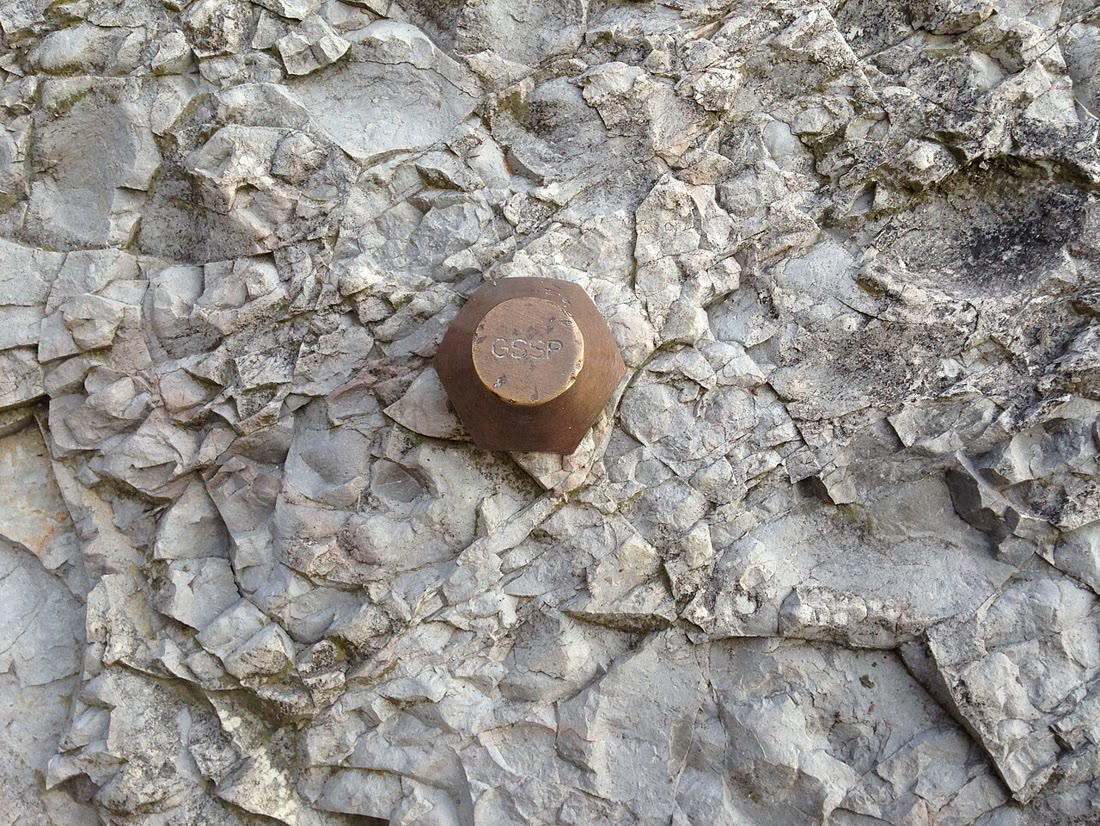
\includegraphics[width=0.62\linewidth]{images/book3/b1-golden-spike-zumaia.jpg}

{\small The golden spike of the Selandian \omterm{def:b1:stratigraphic-scale:chronostratigraphy}{Stage} in the Zumaia section: a bronze
marker stamped GSSP, set at the top of the uppermost limestone bed of one
\omterm{def:b1:stratigraphic-scale:lithostratigraphy}{formation}, at the base of the red marls of the next. (Josugoni, CC~BY-SA~4.0,
via Wikimedia Commons.)}
\label{fig:b1:stratigraphic-scale:zumaia}
\end{omfigure}
% ledger: commons:zumaia-gssp, gssp:selandian

\begin{recall}
In a pile of layers that has not been turned over, each layer is younger than
the one below it; a structure that cuts across rocks is younger than they are;
fossils change from older layers to younger ones in the same order everywhere;
the Earth's history is divided into eras and geological periods, each with an
age in years for its start, gathered in an international chart (Book~1,
grade~7). A \omterm{def:b1:cross-sections:log}{borehole log} records the units met against depth, and correlation
matches the same units from log to log (\cref{def:b1:cross-sections:log}); an
\omterm{def:b1:cross-sections:unconformity}{unconformity} is a surface of erosion or non-deposition
(\cref{def:b1:cross-sections:unconformity}). A \omterm{def:b1:clastic-sediments:facies}{sedimentary facies} is a body of
rock whose characters record its environment of deposition
(\cref{def:b1:clastic-sediments:facies}). The biology volumes describe how
species appear and become extinct, and the few mass extinctions in which a large
share of all species disappeared within a short time.
\end{recall}

\section{Three ways to divide the rocks}\label{sec:b1:stratigraphic-scale:three}

A geologist logging a cliff can divide the same pile of beds in three ways: by
what the rocks are made of, by the fossils they contain, and by the time during
which they were laid down. The three divisions answer different questions, and
their boundaries need not coincide. The rules for naming and defining each kind
of unit are set by international agreement.
% ledger: isg:lithostratigraphy

\begin{definition}[Formation, member, group]\label{def:b1:stratigraphic-scale:lithostratigraphy}
A \emph{lithostratigraphic unit}\index{lithostratigraphic unit} is a body of
rock defined and recognised by its lithology and its position among other
bodies, whatever its age. The primary unit is the
\emph{formation}\index{formation (lithostratigraphic)}: a body of rock distinct
enough from its neighbours to be mapped at the scale of the region, into which
the whole column should be divided. A \emph{member}\index{member
(lithostratigraphic)} is a named subdivision of a formation, distinguished by its
lithology; a \emph{group}\index{group (lithostratigraphic)} is a succession of
two or more formations with significant lithological characters in common. A
formal name joins a local geographical name to the rank or to the dominant rock:
the Kell Sandstone, the Mardon Shale Formation.
\end{definition}
% ledger: isg:lithostratigraphy

A \omterm{def:b1:stratigraphic-scale:lithostratigraphy}{formation} may be less than a metre thick or several thousand metres. It is
extended away from its type section only as far as its lithology can be
recognised, so that its boundaries follow the rock, not time.
% ledger: isg:lithostratigraphy

\begin{definition}[Biozone, index fossil, first appearance datum]\label{def:b1:stratigraphic-scale:biozone}
A \emph{biozone}\index{biozone} is a body of strata defined or characterised by
the fossils it contains. A \emph{range zone}\index{range zone} holds the known occurrences of one
taxon; an \emph{interval zone}\index{interval zone} is the body of strata between two specified
fossil horizons, for example the lowest occurrences of two taxa. The
\emph{first appearance datum}\index{first appearance datum} (FAD) of a taxon is
the horizon of its lowest occurrence, the \emph{last appearance
datum}\index{last appearance datum} that of
its highest. An \emph{index fossil}\index{index fossil} is a taxon used to
recognise a biozone: the best are widespread, abundant, easy to identify and
short-lived.
\end{definition}
% ledger: isg:biostratigraphy, og:stratigraphy-principles

A fossil horizon has no thickness; a \omterm{def:b1:stratigraphic-scale:biozone}{biozone} may be a few metres or a few hundred
thick depending on how fast the sediment accumulated while the taxa lived.
Because species evolve and never reappear once extinct, the assemblage of any one
age is unique. Some of the best \omterm{def:b1:stratigraphic-scale:biozone}{index fossils} are microfossils, such as
foraminifera and conodonts: widespread, abundant, and small enough to be
recovered from the cuttings of a well.
% ledger: isg:biostratigraphy, og:stratigraphy-principles

\begin{definition}[Chronostratigraphic and geochronologic units]\label{def:b1:stratigraphic-scale:chronostratigraphy}
A \emph{chronostratigraphic unit}\index{chronostratigraphic unit} is the body of
all the rocks formed during a given interval of geological time, and only during
it; its boundaries are surfaces of equal age. The interval of time itself is a
\emph{geochronologic unit}\index{geochronologic unit}. The ranks, from the
smallest, are the \emph{stage}\index{stage (chronostratigraphic)} (its time:
an age), the \emph{series}\index{series (chronostratigraphic)} (an epoch), the
\emph{system}\index{system (chronostratigraphic)} (a period), the erathem (an
era) and the eonothem (an eon); each unit is made of several consecutive units of
the rank below.
\end{definition}
% ledger: isg:chronostratigraphy

The two words describe the same division seen as rock or as time
(\cref{tab:b1:stratigraphic-scale:ranks}): rocks of the Jurassic \omterm{def:b1:stratigraphic-scale:chronostratigraphy}{System} were
laid down during the Jurassic Period, and the Lower Jurassic \omterm{def:b1:stratigraphic-scale:chronostratigraphy}{Series} during the
Early Jurassic Epoch. The \omterm{def:b1:stratigraphic-scale:chronostratigraphy}{stage} is the smallest unit recognised all over the
world.
% ledger: isg:chronostratigraphy, chart:danian

\begin{table}[htbp]
\centering
\begin{tabular}{lll}
\hline
\omterm{def:b1:stratigraphic-scale:chronostratigraphy}{chronostratigraphic unit} (rock) & \omterm{def:b1:stratigraphic-scale:chronostratigraphy}{geochronologic unit} (time) & example \\
\hline
eonothem & eon    & Phanerozoic \\
erathem  & era    & Cenozoic \\
\omterm{def:b1:stratigraphic-scale:chronostratigraphy}{system}   & period & Paleogene \\
\omterm{def:b1:stratigraphic-scale:chronostratigraphy}{series}   & epoch  & Paleocene \\
\omterm{def:b1:stratigraphic-scale:chronostratigraphy}{stage}    & age    & Danian (\qtyrange{66.00}{61.66}{\Ma}) \\
\hline
\end{tabular}
\caption{The ranks of the chronostratigraphic and \omterm{def:b1:stratigraphic-scale:chronostratigraphy}{geochronologic units}, with the
units that contain the Danian, the first \omterm{def:b1:stratigraphic-scale:chronostratigraphy}{stage} of the Cenozoic.}
\label{tab:b1:stratigraphic-scale:ranks}
\end{table}
% ledger: isg:chronostratigraphy, chart:danian

\section{The principles and correlation}\label{sec:b1:stratigraphic-scale:principles}

Before any rock could be dated in years, the order of events was read from the
rocks themselves. The basic principles of stratigraphy were set out in 1669 by
Nicolas Steno; between 1785 and 1800 Hutton and William Smith added the use
of the layers as intervals of time and of their fossils to recognise them.
% ledger: og:stratigraphy-principles, usgs:hutton-smith

\begin{definition}[Principles of stratigraphy]\label{def:b1:stratigraphic-scale:principles}
\begin{enumerate}
  \item The \emph{principle of superposition}\index{superposition, principle
        of}: in a sequence of sedimentary layers that has not been overturned,
        each layer is younger than the one on which it rests.
  \item The \emph{principle of original horizontality}\index{original
        horizontality, principle of}: sediments and lava flows are laid down
        horizontally, or nearly so --- slightly sloping at the edges of a
        basin.
  \item The \emph{principle of lateral continuity}\index{lateral continuity,
        principle of}: within a basin, a layer extends continuously in every
        direction until it thins out at the basin's edge or against an
        obstacle; a layer cut by a valley continues on the other side.
  \item The \emph{principle of cross-cutting relationships}\index{cross-cutting
        relationships, principle of}: a body or structure that cuts across
        rocks --- a dyke, a fault, an erosion surface --- is younger than the
        rocks it cuts.
  \item The \emph{principle of faunal succession}\index{faunal succession,
        principle of}: fossil taxa succeed one another in the same order in
        every region, so that rocks holding the same assemblage are of the same
        age.
\end{enumerate}
\end{definition}
% ledger: og:stratigraphy-principles, eli:relative-dating, usgs:fossil-succession, isg:chronostratigraphy

The principles are not equally strong. Superposition gives an order that every
other method must respect. Original horizontality is what makes a tilted bed a
record of later deformation. Lateral continuity is what allows a geologist to
draw the same layer on both sides of a valley, and, within a limited distance, a
bedding plane traced on the ground is the best line of equal age there is.
Faunal succession is the one that crosses oceans; it is the subject of the next
paragraphs.
% ledger: isg:chronostratigraphy, og:stratigraphy-principles

\subsection*{Correlation by biozones}

\omterm{def:b1:cross-sections:log}{Correlation} by fossils compares the order of first and last appearances in two
sections (figure below). The two are not equally reliable. The highest fossil of
a taxon found in a section depends on how many were preserved: where they are
rare, the last one found may lie well below the level at which the taxon really
disappeared, and a fossil eroded and redeposited can turn up above it. A first
appearance can be displaced too, but a widespread taxon that spread quickly is
reached at much the same level across a basin.
% ledger: isg:biostratigraphy

\begin{omfigure}
\begin{tikzpicture}[font=\footnotesize, y=0.13cm]
  % section 1: 40 m, sandstone 0-14, shale 14-40
  \fill[lith sandstone] (0,0) rectangle (0.8,14);
  \fill[lith shale] (0,14) rectangle (0.8,40);
  \draw[black!70] (0,0) rectangle (0.8,40);
  \node[anchor=south, font=\small] at (1.4,41.5) {section 1};
  \foreach \x/\a/\b/\t in {1.1/0/27/a, 1.4/10/34/b, 1.7/20/40/c, 2.0/30/40/d} {
    \draw[line width=2.2pt, omThm] (\x,\a) -- (\x,\b);
    \node[anchor=base, font=\scriptsize] at (\x,-4.5) {\t};
  }
  \foreach \y/\z in {5/a, 15/b, 25/c, 35/d}
    \node[anchor=east, font=\scriptsize] at (-0.1,\y) {zone \z};
  \foreach \y in {10,20,30} \draw[black!50] (-1.3,\y) -- (0,\y);
  % scale bar
  \draw[thick] (-1.5,0) -- (-1.5,10) node[midway, anchor=east, font=\scriptsize] {\qty{10}{m}};
  % section 2: 24 m, sandstone 0-3, shale 3-24
  \begin{scope}[xshift=7cm]
    \fill[lith sandstone] (0,0) rectangle (0.8,3);
    \fill[lith shale] (0,3) rectangle (0.8,24);
    \draw[black!70] (0,0) rectangle (0.8,24);
    \node[anchor=south, font=\small] at (1.4,25.5) {section 2};
    \foreach \x/\a/\b/\t in {1.1/0/13/a, 1.4/6/20/b, 1.7/12/24/c, 2.0/18/24/d} {
      \draw[line width=2.2pt, omThm] (\x,\a) -- (\x,\b);
      \node[anchor=base, font=\scriptsize] at (\x,-4.5) {\t};
    }
    \foreach \y/\z in {3/a, 9/b, 15/c, 21/d}
      \node[anchor=west, font=\scriptsize] at (2.3,\y) {zone \z};
    \foreach \y in {6,12,18} \draw[black!50] (0.8,\y) -- (2.3,\y);
  \end{scope}
  % correlation of the first appearances
  \foreach \u/\v/\t in {10/6/b, 20/12/c, 30/18/d}
    \draw[densely dashed, omThm!70!black] (2.15,\u) -- (6.85,\v)
      node[pos=0.5, fill=white, inner sep=1pt, font=\scriptsize] {FAD \t};
\end{tikzpicture}

{\small A range chart and a correlation by \omterm{def:b1:stratigraphic-scale:biozone}{biozones} (invented taxa \emph{a} to
\emph{d}). The thick bars are the ranges of the taxa in each section. Three
\omterm{def:b1:stratigraphic-scale:biozone}{interval zones} are bounded by the first appearances of \emph{b}, \emph{c} and
\emph{d}, which are joined from section to section (dashed). The last
appearance of \emph{a} falls in the upper part of zone~\emph{c} in section~1
and near its base in section~2: it is a poorer guide. The zones are thinner in
section~2, where the sediment accumulated more slowly.}
\label{fig:b1:stratigraphic-scale:range-chart}
\end{omfigure}

\begin{method}[Correlating sections by biozones]\label{met:b1:stratigraphic-scale:biozones}
\begin{enumerate}
  \item Plot, for each section, the range of each taxon against height: from
        its lowest to its highest occurrence.
  \item Choose the fossil horizons that define the zones --- preferably first
        appearances of widespread taxa that are independent of the facies.
  \item Draw the zone boundaries in each section at these horizons.
  \item Join the same horizons from section to section; check that the lines
        do not cross, as superposition requires.
  \item Read, between two lines, the thickness of each zone in each section;
        where a zone is missing, look for an \omterm{def:b1:cross-sections:unconformity}{unconformity} or a change of
        facies before concluding that the taxon is absent.
\end{enumerate}
\end{method}

A \omterm{def:b1:stratigraphic-scale:biozone}{biozone} is only as good as the independence of its fossils from the
environment. A bivalve that lived only on sandy shores is found only in
sandstones; following it from section to section follows the sandstone, not
time. Biostratigraphic correlation is therefore not necessarily time
correlation: it may follow a facies whose age changes from place to place.
% ledger: isg:biostratigraphy

\subsection*{Boundaries that cross time}

Different sediments are laid down at the same time in different places: sand on
the shore, mud offshore, lime farther out on a shelf starved of sand. A line of
equal age therefore passes from one lithology to another. Conversely, a
lithological boundary traced across a basin need not be a line of equal age at
all.
% ledger: og:stratigraphy-principles, isg:chronostratigraphy

\begin{definition}[Diachronous boundary]\label{def:b1:stratigraphic-scale:diachronous}
A boundary is \emph{diachronous}\index{diachronous boundary} when its age
changes from place to place along it. The boundaries of \omterm{def:b1:stratigraphic-scale:lithostratigraphy}{formations} and of
facies are commonly diachronous; the boundaries of \omterm{def:b1:stratigraphic-scale:chronostratigraphy}{chronostratigraphic units}
are, by definition, not.
\end{definition}
% ledger: isg:lithostratigraphy, isg:chronostratigraphy, isg:biostratigraphy

The classic case is a transgression: \omterm{def:b1:diagenesis-basins:eustasy}{relative sea level} rises faster than
sediment can fill the room made, and the shoreline moves inland. The beach sand
is laid down at the shoreline at every instant, so a sheet of sandstone spreads
inland with it; the offshore mud follows on top. The top of the sandstone is
then the trace of the moving shoreline: young inland, old seaward
(figure below). The order of facies seen in one vertical section --- sandstone
under shale under limestone --- repeats their order across the shelf at one
instant; the Year~3 volume makes this the basis of its facies models.
% ledger: og:stratigraphy-principles, isg:lithostratigraphy

\begin{omfigure}
\begin{tikzpicture}[font=\footnotesize, x=1cm, y=1cm]
  % basement surface B(x) = 1.6 (1 - x/14), rising towards the land on the left
  \fill[lith granite] (0,-0.5) -- (0,1.6) -- (14,0) -- (14,-0.5) -- cycle;
  \fill[lith sandstone] (0,1.6) -- (14,0) -- (14,0.5) -- (0,2.1) -- cycle;
  \fill[lith shale] (0,2.1) -- (14,0.5) -- (14,1.5) -- (0,3.1) -- cycle;
  \fill[lith limestone] (0,3.1) -- (14,1.5) -- (14,3.6) -- (0,3.6) -- cycle;
  \draw[unconformity] (0,1.6) -- (14,0);
  \draw[black!70] (0,2.1) -- (14,0.5) (0,3.1) -- (14,1.5);
  \draw[black!70] (0,-0.5) rectangle (14,3.6);
  % time lines: horizontal, from the basement (or the left edge) to the right edge
  \foreach \y/\t in {0.6/1, 1.1/2, 1.6/3, 2.1/4, 2.6/5, 3.1/6} {
    \pgfmathsetmacro{\xs}{max(0, 14*(1-\y/1.6))}
    \draw[omThm, thick, densely dashed] (\xs,\y) -- (14,\y) node[anchor=west, text=black] {$t_\t$};
  }
  % two sections
  \foreach \x/\n in {3/1, 11/2} {
    \draw[very thick, black] (\x,-0.5) -- (\x,3.6);
    \node[anchor=south, font=\small] at (\x,3.65) {section \n};
  }
  \node[fill=white, inner sep=1pt, font=\scriptsize] at (5.6,1.21) {sandstone};
  \node[fill=white, inner sep=1pt] at (12.6,1.2) {shale};
  \node[fill=white, inner sep=1pt] at (7.0,3.25) {limestone};
  \node[fill=white, inner sep=1pt] at (12.0,-0.25) {basement};
  \draw[-{Stealth}, thick] (5.6,4.35) -- (3.6,4.35) node[anchor=east] {land};
  \draw[-{Stealth}, thick] (8.4,4.35) -- (10.4,4.35) node[anchor=west] {sea};
\end{tikzpicture}

{\small A sandstone sheet laid down during a transgression (schematic, vertical
scale exaggerated). The dashed lines $t_1$ to $t_6$ join points of equal age,
$t_1$ the oldest. Where one meets the basement, it starts at the shoreline of
its time; seaward it passes from sand to mud and, in the younger ones, to lime.
The top of the sandstone
lies between $t_1$ and $t_2$ in section~2 but between $t_3$ and $t_4$ in
section~1: the \omterm{def:b1:stratigraphic-scale:lithostratigraphy}{formation} boundary is \omterm{def:b1:stratigraphic-scale:diachronous}{diachronous}, younger towards the land.}
\label{fig:b1:stratigraphic-scale:diachronous}
\end{omfigure}

How fast does the boundary's age change along it? On a coastal plain that rises
gently inland, the answer is a matter of geometry.

\begin{proposition}[Speed of a transgression]\label{prop:b1:stratigraphic-scale:transgression}
A coastal plain rises inland with the uniform slope $s$, and the \omterm{def:b1:diagenesis-basins:eustasy}{relative sea
level} rises at the constant rate $R$, with no sediment added at the shore. The
shoreline then moves inland at the speed
\[
  u = \frac{R}{s},
\]
and a boundary that follows the shoreline is younger, at a point a distance $d$
farther inland, by $\Delta t = d/u = d\,s/R$.
\end{proposition}

\begin{proof}
Take $x$ as the distance inland from a fixed point and $z$ as the height; the
plain is the line $z = s x$, and the sea surface at time $t$ is
$z = z_0 + R t$. The shoreline is where they meet: $s\,x(t) = z_0 + R t$, so
$x(t) = (z_0 + R t)/s$ and $\mathrm dx/\mathrm dt = R/s$. The shoreline reaches
a point a distance $d$ farther inland after the time $d/u = d\,s/R$.
\end{proof}

The ratio is large because coastal plains are nearly flat. A rise of
\qty{10}{m} per million years over a plain sloping $1$ in $2000$ moves the shore
\qty{20}{km} inland per million years; a sandstone top that looks like one
surface in a cliff is then a million years younger \qty{20}{km} inland. Sediment
brought to the shore slows the transgression or reverses it.

\subsection*{Lines of equal age}

What correlates time, then, if lithology does not and fossils only
approximately? The best lines are made by events that leave a trace everywhere
at once. A volcanic ash falls over a wide area in what is, geologically, an
instant, and settles on sand, mud and lime alike: an ash bed is a line of equal
age that crosses facies boundaries, and it can often be dated in years by the
methods of \cref{ch:b1:radiometric-methods}. Reversals of the Earth's magnetic
field, taken up in the Year~3 volume, are recorded in rocks of many kinds and can
be recognised worldwide once their order is known; so are sharp shifts in the
isotopes of carbon, such as the one that marks the base of the Ypresian
(\cref{tab:b1:stratigraphic-scale:gssps}). Between two
dated levels, the age of any bed is estimated by assuming that the sediment
accumulated at a constant rate.
% ledger: isg:chronostratigraphy

\begin{proposition}[Age between two dated levels]\label{prop:b1:stratigraphic-scale:interpolation}
Two beds at the heights $z_1 < z_2$ of a continuous section have the ages
$t_1 > t_2$. If the sediment accumulated at a constant rate between them, a
level at the height $z$ between them has the age
\[
  t = t_1 - f\,(t_1 - t_2), \qquad f = \frac{z - z_1}{z_2 - z_1},
\]
and the rate of accumulation is $r = (z_2 - z_1)/(t_1 - t_2)$. If the two ages
carry the independent standard uncertainties $\sigma_1$ and $\sigma_2$, the
interpolated age carries the uncertainty
\[
  \sigma_t = \sqrt{(1 - f)^2 \sigma_1^2 + f^2 \sigma_2^2}.
\]
\end{proposition}

\begin{proof}
At a constant rate $r$, the height grows linearly with time: $z - z_1 = r\,(t_1
- t)$, since ages decrease upwards. At $z_2$, $z_2 - z_1 = r\,(t_1 - t_2)$, which
gives $r$; dividing the two relations gives $t_1 - t = f\,(t_1 - t_2)$. The age
is the linear combination $t = (1 - f)\,t_1 + f\,t_2$ of two independent
quantities; the variance of $a X + b Y$ for independent $X$ and $Y$ is $a^2
\operatorname{Var} X + b^2 \operatorname{Var} Y$, which gives $\sigma_t$.
\end{proof}

The uncertainty is smallest between the two dated beds and is never larger than
the larger of $\sigma_1$ and $\sigma_2$ there. The real limit is the assumption:
sediment accumulates in pulses, may stop at hidden breaks, and compacts
differently in sand and in mud (\cref{prop:b1:diagenesis-basins:solid}), so that
the interpolated age is no better than the regularity of the section.

\section{Boundary stratotypes}\label{sec:b1:stratigraphic-scale:gssp}

A \omterm{def:b1:stratigraphic-scale:chronostratigraphy}{chronostratigraphic unit} is defined in the rock before it is dated. The older
practice described each \omterm{def:b1:stratigraphic-scale:chronostratigraphy}{stage} by a type section of the whole unit; but the top
of one type section and the base of the next, chosen in different places, could
leave a gap of unassigned time between them or overlap. The modern practice
defines only the lower boundary of each unit at one point in one section; the
upper boundary is the lower boundary of the next unit. No interval of time can
then fall between two units or belong to both.
% ledger: isg:stratotype, isg:chronostratigraphy

\begin{definition}[Boundary stratotype, unit stratotype, GSSP]\label{def:b1:stratigraphic-scale:gssp}
A \emph{stratotype}\index{stratotype} is the designated section of rock that
serves as the standard of reference for a unit or a boundary. A \emph{unit
stratotype}\index{unit stratotype} is the type section of a whole unit; a
\emph{boundary stratotype}\index{boundary stratotype} is the section that
contains the specific point defining a boundary between two units. A
\emph{global boundary stratotype section and point}\index{global boundary
stratotype section and point (GSSP)} (GSSP) is the boundary stratotype of a
unit of the international chronostratigraphic scale: a single point in a single
section, chosen by international agreement, which defines the base of a \omterm{def:b1:stratigraphic-scale:chronostratigraphy}{stage}
and of every larger unit that begins with it.
\end{definition}
% ledger: isg:stratotype, isg:chronostratigraphy, gssp:protocol

The GSSP is a point in rock, not an age. Its age in years is whatever the best
dating of that point gives, and it may be refined without moving the point. The
section is chosen to make the point findable elsewhere: deposition continuous
across the boundary (never at an \omterm{def:b1:cross-sections:unconformity}{unconformity}, where the missing time would make
the boundary ambiguous), preferably marine, rich in well-preserved fossils of
widespread taxa, without a change of facies at the level, little deformed or
altered, accessible and protected. Above all, the point is placed at a level
that coincides with one chosen signal --- usually the first appearance of a
taxon --- inside an interval rich in other signals (ash beds, magnetic
reversals, isotopic shifts) by which the level can be recognised far away. A
permanent marker, the golden spike, is placed at the point.
% ledger: isg:chronostratigraphy, isg:stratotype, gssp:protocol

\begin{inthefield}[How a boundary is chosen]
A boundary is studied by a working group of the subcommission in charge of the
\omterm{def:b1:stratigraphic-scale:chronostratigraphy}{system}, which compares candidate sections, logs them bed by bed, samples their
fossils, ash beds and isotopes, and writes a proposal. A proposal needs a
supermajority --- more than \qty{60}{\%} --- of the voting \omterm{def:b1:stratigraphic-scale:lithostratigraphy}{members} of the
subcommission, about twenty specialists; it then passes to the voting \omterm{def:b1:stratigraphic-scale:lithostratigraphy}{members} of
the International Commission on Stratigraphy, the executive officers and the
chairs of its seventeen subcommissions, and finally to the executive committee of
the International Union of Geological Sciences, whose approval ratifies it. The
results are published, the marker is set in the rock, and no change to a newly
established boundary may be proposed for ten years.
\end{inthefield}
% ledger: gssp:protocol

\begin{table}[htbp]
\centering
\small
\begin{tabular}{>{\raggedright\arraybackslash}p{2.4cm}>{\raggedright\arraybackslash}p{1.2cm}>{\raggedright\arraybackslash}p{3.7cm}>{\raggedright\arraybackslash}p{5.6cm}c}
\hline
base of & age (\unit{\Ma}) & section & marker of the point & ratified \\
\hline
Fortunian (Cambrian) & 538.8 & Fortune Head, Newfoundland, Canada & first appearance of the trace fossil \emph{Trichophycus pedum} & 1992 \\
Lochkovian (Devonian) & 419.62 & Klonk, near Prague, Czech Republic & first appearance of the graptolite \emph{Monograptus uniformis} & 1972 \\
Induan (Triassic) & 251.902 & Meishan, Zhejiang, China & first appearance of the conodont \emph{Hindeodus parvus}, base of Bed~27c & 2001 \\
Danian (Paleogene) & 66.00 & Oued Djerfane, El Kef, Tunisia & base of a \qty{50}{cm} dark boundary clay; iridium anomaly & 1991 \\
Selandian & 61.66 & Zumaia, Spain & base of red marls; second radiation of a nannofossil group & 2008 \\
Ypresian (Eocene) & 56.00 & Dababiya, near Luxor, Egypt & base of a carbon-isotope excursion & 2003 \\
Chibanian & 0.774 & Chiba, Japan & base of a tephra, just below a magnetic reversal & 2020 \\
Meghalayan & 0.0042 & Mawmluh Cave, Meghalaya, India & a level \qty{7.45}{mm} deep in a speleothem & 2018 \\
\hline
\end{tabular}
\caption{Eight GSSPs. The markers are first appearances of taxa, a geochemical
anomaly, an isotope excursion, a magnetic reversal and a climatic event recorded
in a cave deposit.}
\label{tab:b1:stratigraphic-scale:gssps}
\end{table}
% ledger: gssp:fortunian, gssp:lochkovian, gssp:induan, gssp:danian, gssp:selandian, gssp:ypresian, gssp:chibanian, gssp:meghalayan

\Cref{tab:b1:stratigraphic-scale:gssps} shows how varied the chosen signals are.
The Paleozoic and Mesozoic boundaries of the table rest on first appearances of
fossils, a graptolite and a conodont; at the base of the Cambrian the fossil is a
trace fossil, the mark left in the sediment by an animal's activity rather than
the animal itself. In the Cenozoic examples the signals are chemical and
physical: the iridium of the Danian, the carbon-isotope excursion of the Ypresian,
the magnetic reversal that lies \qty{1.1}{m} above the Chibanian point. The
youngest boundary of the table is not in marine rock at all: the base of the
Meghalayan is a level inside a speleothem, a deposit grown in a cave, recording
a climatic event of 4200 years ago.
% ledger: gssp:fortunian, gssp:danian, gssp:ypresian, gssp:chibanian, gssp:meghalayan

\begin{dated}{2026}
% ledger: gssp:count, chart:stage-count
In October 2026 the table of the International Commission on Stratigraphy listed
80 ratified GSSPs, and two more proposed. The first was ratified in 1972, at
Klonk; the most recent in 2024, when two boundaries of the Silurian, until then
defined in Wales, were moved to new sections in Spain and in the Czech
Republic. Of the 101 \omterm{def:b1:stratigraphic-scale:chronostratigraphy}{stages} of the Phanerozoic on the chart, 21 still had no
ratified GSSP; their bases are provisional.
\end{dated}

Below the Phanerozoic, the scale is mostly divided differently. Except for its
youngest \omterm{def:b1:stratigraphic-scale:chronostratigraphy}{system}, the Ediacaran, the Precambrian is cut at round ages chosen by
agreement --- the divisions are defined in years, not by points in rock.
% ledger: isg:chronostratigraphy

\section{Mass extinctions as markers}\label{sec:b1:stratigraphic-scale:extinctions}

The biology volumes describe the mass extinctions as moments when a large share of
species disappeared within a geologically short time. For stratigraphy, such an
event is a gift: a horizon found on every continent and in every ocean,
across which the fossil assemblages change completely. Two of them bound the
three eras of the Phanerozoic.
% ledger: schulte:kpg, burgess:end-permian

\subsection*{The end of the Cretaceous}

In 1980, L.~W.~Alvarez, W.~Alvarez, F.~Asaro and H.~V.~Michel measured iridium
--- one of the platinum metals, depleted in the Earth's \omterm{def:b1:layered-earth:layers}{crust} compared with
their abundance in the cosmos --- in deep-sea limestones across the boundary
between the Cretaceous and the Tertiary --- today the boundary between the
Cretaceous and the Paleogene, the K--Pg boundary. They found it enriched about 30 times above
the background in Italy, 160 times in Denmark and 20 times in New Zealand,
exactly at the level of the extinctions. They proposed that an \omterm{def:b1:comparative-planetology:small-bodies}{asteroid}
$\qty{10}{km}$ across, give or take four, had struck the Earth and thrown about
60 times its own mass of pulverised rock into the atmosphere; the dust would
have spread worldwide and darkened the sky. The clay at the boundary, they
noted, differs chemically from the clay of the limestones above and below.
% ledger: alvarez:iridium

Later work tied the boundary to one impact, Chicxulub. Argon--argon dating
places that impact and the boundary with its extinctions within \num{32000}
years of each other, and a review of the evidence concluded that the impact triggered the
extinction, which also fell within the time of a great outpouring of basalt in
India. The GSSP of the base of the Danian --- the base of the Paleogene and of
the whole Cenozoic --- is placed at the base of the dark boundary clay at El Kef
in Tunisia, at the iridium anomaly. The same boundary can be seen on land, in
Colorado (figure below).
% ledger: renne:kpg, schulte:kpg, gssp:danian, commons:kt-tlsp

\begin{omfigure}
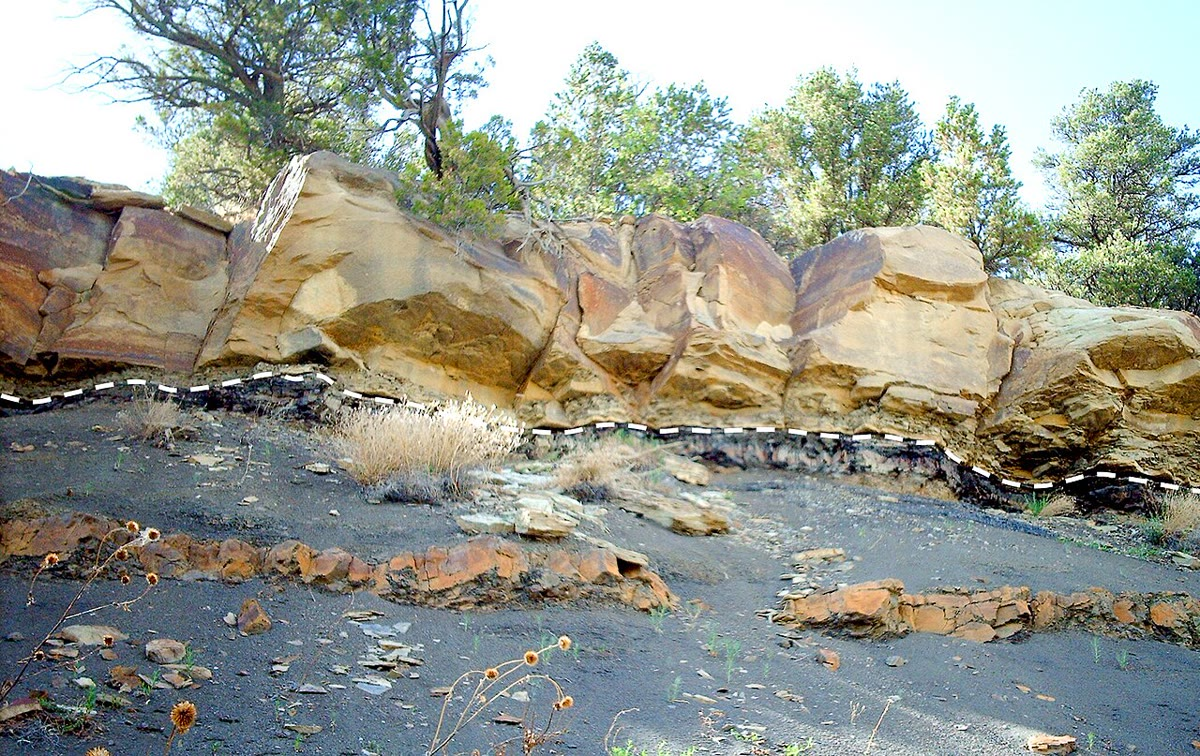
\includegraphics[width=0.78\linewidth]{images/book3/b1-kpg-boundary-trinidad.jpg}

{\small The boundary between the Cretaceous and the Paleogene, marked by the
dashed line, at Trinidad Lake State Park, Colorado: sandstone above, dark beds
below and along the boundary. (Nationalparks, CC~BY-SA~2.5,
via Wikimedia Commons; the dashed line is in the original.)}
\label{fig:b1:stratigraphic-scale:kpg}
\end{omfigure}
% ledger: commons:kt-tlsp

\subsection*{The end of the Permian}

The extinction at the end of the Permian was the most severe loss of marine and
land life of the last half-billion years. At Meishan in China, the section that
holds the GSSP of the base of the Triassic, five ash beds have been dated by the
uranium--lead method on zircon. They place the extinction between
\qty[uncertainty-mode=separate]{251.941(37)}{\Ma} and \qty[uncertainty-mode=separate]{251.880(31)}{\Ma}: an interval of
\num[uncertainty-mode=separate]{60 \pm 48} thousand years. A sharp negative shift of \qty{3}{\permil} in
the carbon isotopes of the carbonates precedes it, and the carbon cycle remained
unstable for about \num{500} thousand years.
% ledger: burgess:end-permian, gssp:induan

The base of the Triassic itself, \qty[uncertainty-mode=separate]{251.902(24)}{\Ma}, is not placed at the
extinction but at the first appearance of the conodont \emph{Hindeodus parvus},
a level that falls within the interval of the extinction dated at Meishan. An
extinction is a set of last appearances, which preservation blurs; one first
appearance of a well-known species makes a sharper line. The causes of the two extinctions ---
an impact, the great basalt provinces --- are the subject of the Year~2 volume.
% ledger: gssp:induan, isg:biostratigraphy, burgess:end-permian

\section{The international chart}\label{sec:b1:stratigraphic-scale:chart}

The International Chronostratigraphic Chart gathers all the units, from the
eonothems to the \omterm{def:b1:stratigraphic-scale:chronostratigraphy}{stages}, in one table: their names, the base of each in millions
of years with its uncertainty, a mark for each base defined by a ratified GSSP,
and a standard colour for each unit, that of the Commission for the Geological
Map of the World. The
Phanerozoic part, reduced to its eras and periods, is drawn below from the
chart's own values.
% ledger: ics:base.Paleozoic, ics:colour.Paleozoic, gssp:count

\begin{omfigure}
\begin{tikzpicture}[font=\footnotesize]
\begin{axis}[y dir=reverse, ymin=0, ymax=538.8, xmin=0, xmax=6.2,
  width=6.6cm, height=11cm, scale only axis, clip=false,
  axis x line=none, axis y line*=left, ytick={0,100,...,500},
  ylabel={age (\unit{\Ma})}, tick label style={font=\scriptsize}]
  \pgfplotsinvokeforeach{Paleozoic,Mesozoic,Cenozoic,Cambrian,Ordovician,Silurian,Devonian,Carboniferous,Permian,Triassic,Jurassic,Cretaceous,Paleogene,Neogene,Quaternary}{
    \addplot[fill=ics#1, draw=black!70, line width=0.3pt] table[x=x, y=age] {figdata/out/bachelor-1-ics_chart-bar-#1.dat};}
  \addplot[draw=none, nodes near coords, point meta=explicit symbolic,
    every node near coord/.style={anchor=center, rotate=90, font=\scriptsize\bfseries}]
    table[x=x, y=age, meta=name] {figdata/out/bachelor-1-ics_chart-eras.dat};
  \addplot[draw=none, nodes near coords, point meta=explicit symbolic,
    every node near coord/.style={anchor=center, font=\scriptsize}]
    table[x=x, y=age, meta=name] {figdata/out/bachelor-1-ics_chart-periods.dat};
  \addplot[mark=-, mark size=3pt, only marks, nodes near coords, point meta=explicit symbolic,
    every node near coord/.style={anchor=west, xshift=1pt, font=\scriptsize}]
    table[x=x, y=age, meta=lab] {figdata/out/bachelor-1-ics_chart-bases.dat};
  \addplot[only marks, mark=triangle*, mark size=3pt, mark options={rotate=90, fill=omThm, draw=omThm},
    nodes near coords, point meta=explicit symbolic,
    every node near coord/.style={anchor=west, xshift=3pt, font=\scriptsize, text=omThm}]
    table[x expr=\thisrow{x}+1.75, y=age, meta=name] {figdata/out/bachelor-1-ics_chart-events.dat};
  \node[anchor=south, font=\scriptsize] at (axis cs:2,0) {Quaternary};
  \node[anchor=west, font=\scriptsize] at (axis cs:3.0,-14) {0};
  \node[anchor=south, font=\scriptsize\itshape] at (axis cs:0.5,-30) {era};
  \node[anchor=south, font=\scriptsize\itshape] at (axis cs:2,-30) {period};
  \node[anchor=south, font=\scriptsize\itshape] at (axis cs:3.5,-30) {base (\unit{\Ma})};
\end{axis}
\end{tikzpicture}

{\small The Phanerozoic on the international chart: its three eras and twelve
periods, to scale, in the chart's colours, with the age of the base of each
period (uncertainties omitted). The triangles mark the two bases that are mass
extinction horizons. The Quaternary, \qty{2.58}{\Ma} long, is the thin band at
the top.}
\label{fig:b1:stratigraphic-scale:chart}
\end{omfigure}
% computed in figdata/bachelor-1/ics_chart.py; ledger: ics:base.Cambrian, ics:colour.Cambrian (every ics base and colour row of the eras and periods), burgess:end-permian, alvarez:iridium

The periods are very unequal (figure above). The Cretaceous lasted
\qty{77.1}{\Myr}, the Neogene \qty{20.46}{\Myr} and the Quaternary only
\qty{2.58}{\Myr}; the mean of the twelve is \qty{44.9}{\Myr}. The inequality is
inherited: the \omterm{def:b1:stratigraphic-scale:chronostratigraphy}{systems} were named in early classifications, before any rock was
dated in years --- some names give a position (Paleogene, Neogene, Quaternary),
some a rock (Carboniferous, Cretaceous), some a people or a place (Ordovician,
Silurian, Devonian, Permian) --- and the chart keeps the names while defining
their bases by GSSPs. The ages in years come from the isotopic dating of
volcanic rocks close to the boundaries, such as the ash beds of Meishan
(\cref{ch:b1:radiometric-methods}), interpolated as in
\cref{prop:b1:stratigraphic-scale:interpolation}; a new version of the chart may
shift an age while the GSSP stays where it is.
% ledger: ics:base.Cretaceous, ics:base.Neogene, ics:base.Quaternary, isg:chronostratigraphy, burgess:end-permian

\begin{dated}{2024}
% ledger: iugs:anthropocene
The Anthropocene, a name proposed in 2001 for a new interval marked by human
activity, was studied from 2009 by a working group of the Subcommission on
Quaternary Stratigraphy. In late 2023 the group proposed a \omterm{def:b1:stratigraphic-scale:chronostratigraphy}{series} beginning
about 1950, with its GSSP in the sediment of Crawford Lake, Ontario. The
subcommission's vote, closed on 4 March 2024, rejected it: 4 votes for, 12
against, 3 abstentions, 3 \omterm{def:b1:stratigraphic-scale:lithostratigraphy}{members} not voting. The voting \omterm{def:b1:stratigraphic-scale:lithostratigraphy}{members} of the
International Commission on Stratigraphy recognised the vote. The Anthropocene
is not a unit of the chart; it remains an informal term, widely used.
\end{dated}

\section{Exercises}

\begin{exercise}[$\star$]\label{exo:b1:stratigraphic-scale:1}
Say whether each name is that of a lithostratigraphic, a biostratigraphic, a
chronostratigraphic or a \omterm{def:b1:stratigraphic-scale:chronostratigraphy}{geochronologic unit}, and give its rank where it has
one: (a)~the Jurassic \omterm{def:b1:stratigraphic-scale:chronostratigraphy}{System}; (b)~the Mardon Shale \omterm{def:b1:stratigraphic-scale:lithostratigraphy}{Formation}; (c)~the Early
Cretaceous; (d)~the \emph{Hindeodus parvus} Zone; (e)~the Danian \omterm{def:b1:stratigraphic-scale:chronostratigraphy}{Stage};
(f)~the Paleocene Epoch; (g)~a sandstone \omterm{def:b1:stratigraphic-scale:lithostratigraphy}{member} of the Mardon Shale.
% ledger: isg:lithostratigraphy, isg:biostratigraphy, isg:chronostratigraphy
\end{exercise}

\begin{exercise}[$\star$]\label{exo:b1:stratigraphic-scale:2}
With the bases of the eras in the figure of the chart (those of the Cambrian,
the Triassic and the Paleogene), compute the duration of
the Paleozoic, the Mesozoic and the Cenozoic, and the share of the Phanerozoic
that each represents. What share of the time since the base of the Hadean,
\qty{4567}{\Ma}, does the whole Phanerozoic represent?
% ledger: ics:base.Paleozoic, ics:base.Mesozoic, ics:base.Cenozoic, ics:base.Hadean
\end{exercise}

\begin{exercise}[$\star$]\label{exo:b1:stratigraphic-scale:3}
A cliff shows, from the bottom: beds A, B, C and D, tilted at \ang{40}; a dyke
E that cuts A to D; an erosion surface that cuts the top of D and the dyke;
horizontal beds F and G above it; a fault that offsets A to F but not G. Put the
events in order, and name the principle that justifies each step.
\end{exercise}

\begin{exercise}[$\star$]\label{exo:b1:stratigraphic-scale:4}
Two ash beds \qty{30}{m} apart in a shale are dated \qty{85.40}{\Ma} (the lower)
and \qty{84.60}{\Ma} (the upper). The first appearance of an \omterm{def:b1:stratigraphic-scale:biozone}{index fossil} lies
\qty{12}{m} above the lower ash. Compute the rate of accumulation and the age of
the first appearance, assuming the rate constant.
\end{exercise}

\begin{exercise}[$\star\star$]\label{exo:b1:stratigraphic-scale:5}
In a section, four taxa have the ranges (heights in metres): A 0--34, B
12--50, C 26--62, D 41--70. (a)~Draw the range chart. (b)~Give the extent and
the thickness of the concurrent-range zone of B and C, and of the \omterm{def:b1:stratigraphic-scale:biozone}{interval zone}
between the first appearances of B and D. (c)~In a second section, B is found
from 3 to 15~m and C from 9 to 22~m, and nothing else is known. Which zone
boundaries of (b) can be recognised there, and which cannot? Which horizons can
be correlated between the two sections with the most confidence?
\end{exercise}

\begin{exercise}[$\star\star$]\label{exo:b1:stratigraphic-scale:6}
During a transgression the shoreline moved inland at \qty{20}{km} per million
years. (a)~By how much does the age of the top of the shoreline sandstone differ
between two wells \qty{60}{km} apart along the direction of the transgression?
(b)~An ash falls one million years after the shoreline passed the seaward well,
where the offshore mud accumulates at \qty{30}{m} per million years. How far
above the top of the sandstone is the ash bed found there? (c)~Where was the
shoreline when the ash fell? Is the ash found above or below the sandstone in
the landward well, and why may it not be found there at all? Explain with a
sketch.
\end{exercise}

\begin{exercise}[$\star\star$]\label{exo:b1:stratigraphic-scale:7}
(a)~Compute the relative uncertainty of the ages of the bases of the Lochkovian
(\qty[uncertainty-mode=separate]{419.62(136)}{\Ma}) and of the Induan (\qty[uncertainty-mode=separate]{251.902(24)}{\Ma}), in per
cent. Suggest why they differ so much. (b)~From the two ages that bracket the
end-Permian extinction at Meishan, \qty[uncertainty-mode=separate]{251.941(37)}{\Ma} and
\qty[uncertainty-mode=separate]{251.880(31)}{\Ma}, recompute the duration of the extinction and its
uncertainty, assuming the two errors independent. Compare with the published
\num[uncertainty-mode=separate]{60 \pm 48} thousand years.
% ledger: ics:base.Devonian, gssp:induan, burgess:end-permian
\end{exercise}

\begin{exercise}[$\star\star$]\label{exo:b1:stratigraphic-scale:8}
Take the \omterm{def:b1:comparative-planetology:small-bodies}{asteroid} of 1980 as a sphere \qty{10}{km} across, of density
\qty{3000}{kg.m^{-3}} (an assumed value), throwing up 60 times its mass as dust.
(a)~Compute the mass of the \omterm{def:b1:comparative-planetology:small-bodies}{asteroid} and of the dust. (b)~Spread the dust evenly
over the Earth (diameter \qty{12756}{km}): what mass falls on each square metre?
(c)~Laid down at a density of \qty{2500}{kg.m^{-3}}, how thick is the layer?
(d)~Repeat (c) for diameters of \qty{6}{km} and \qty{14}{km}, the range of the
estimate. Compare with the thickness of the boundary clay at the Danian GSSP.
% ledger: alvarez:iridium, planet:Earth.diameter, gssp:danian
\end{exercise}

\begin{exercise}[$\star\star$]\label{exo:b1:stratigraphic-scale:9}
(a)~In a condensed section where sediment accumulated at \qty{2}{m} per million
years, how thick is the interval of \num{60} thousand years of the end-Permian
extinction? How thick would it be for the shortest and the longest durations
allowed by its uncertainty? (b)~In a deep-sea section accumulating at
\qty{10}{m} per million years, how thick is the interval of \num{32000} years
within which the impact and the K--Pg boundary are synchronous? (c)~What do
these numbers say about sampling a section to study an extinction?
% ledger: burgess:end-permian, renne:kpg
\end{exercise}

\begin{exercise}[$\star\star\star$]\label{exo:b1:stratigraphic-scale:10}
A coastal plain slopes $1$ in $2000$ and the \omterm{def:b1:diagenesis-basins:eustasy}{relative sea level} rises at
\qty{10}{m} per million years. (a)~With
\cref{prop:b1:stratigraphic-scale:transgression}, how fast does the shoreline
move inland, and by how much does the age of the top of the shoreline sandstone
differ between two wells \qty{30}{km} apart? (b)~Sediment is now delivered to the
shore, which builds the coastal plain upward by $a$ metres per million years at
the shoreline. Show that the shoreline moves inland at $(R - a)/s$ as long as
$a < R$. What happens when $a > R$? (c)~Explain why a sandstone top whose age
changes by a million years can look, in a single cliff, exactly like a surface of
equal age.
\end{exercise}

\begin{exercise}[$\star\star\star$]\label{exo:b1:stratigraphic-scale:11}
Two ash beds lie at \qty{10}{m} and \qty{50}{m} in a section and are dated
\qty[uncertainty-mode=separate]{100.50(5)}{\Ma} and \qty[uncertainty-mode=separate]{99.70(3)}{\Ma}. (a)~Interpolate the age of a level
at \qty{25}{m} and its uncertainty with
\cref{prop:b1:stratigraphic-scale:interpolation}. (b)~Where between the two ashes
is the uncertainty smallest? Find the value of $f$ that minimises $\sigma_t$, and
the minimum. (c)~Show that $\sigma_t$ never exceeds the larger of $\sigma_1$ and
$\sigma_2$ between the two beds.
\end{exercise}

\begin{exercise}[$\star\star\star$]\label{exo:b1:stratigraphic-scale:12}
A well passes through a uniform shale. An ash dated \qty{30.0}{\Ma} lies at
\qty{1000}{m} depth and an ash dated \qty{29.0}{\Ma} at \qty{200}{m}; a \omterm{def:b1:stratigraphic-scale:chronostratigraphy}{stage}
boundary lies at \qty{600}{m}. (a)~Interpolate its age from the depths. (b)~The
grains, not the pores, arrived at a constant rate. Using the shale of
\cref{tab:b1:diagenesis-basins:athy} and
\cref{prop:b1:diagenesis-basins:solid}, compute the solid thickness between each
ash and the boundary, and interpolate the age again in proportion to it.
(c)~By how many thousand years do the two estimates differ, and which is the
better?
% ledger: pybacktrack:compaction
\end{exercise}

\section{Problem: Correlating three sections across a basin}

\begin{problem}[{Weekend problem --- how fossils, ash beds and a diachronous
sandstone combine to date a stage boundary}]
\label{pb:b1:stratigraphic-scale:1}
% values: calc/ch24.py; the basin, its sections, its taxa (Vardenoceras and Ostreola) and its ash ages are invented
Three sections are logged along a line across an invented basin: A in the west,
B \qty{25}{km} east of A, and C \qty{20}{km} east of B. In each, the Kell
Sandstone is overlain by the Mardon Shale. Heights are in metres above the base
of each section:
\begin{center}
\small
\begin{tabular}{lccc}
\hline
 & A & B & C \\
\hline
total thickness logged                       & 80.0 & 66.0 & 32.0 \\
top of the Kell Sandstone                    & 45.0 & 20.0 & 6.0 \\
ash bed 1 (dated \qty[uncertainty-mode=separate]{152.40(4)}{\Ma})       & 5.0  & 8.0  & 3.0 \\
ash bed 2 (dated \qty[uncertainty-mode=separate]{151.20(4)}{\Ma})       & 71.0 & 56.0 & 27.0 \\
first appearance of \emph{Vardenoceras medium} & 36.6 & 31.2 & 14.8 \\
first appearance of \emph{Vardenoceras ultimum} & 65.8 & 52.0 & 24.8 \\
last appearance of \emph{Vardenoceras primum}   & 49.0 & 40.0 & 19.0 \\
\hline
\end{tabular}
\end{center}
\emph{V.~primum} is found from the base of every section. The bivalve
\emph{Ostreola} is found only in the Kell Sandstone, in all three sections. Three
\omterm{def:b1:stratigraphic-scale:biozone}{interval zones} are defined: zone~1 up to the first appearance of
\emph{V.~medium}, zone~2 up to that of \emph{V.~ultimum}, zone~3 above. A \omterm{def:b1:stratigraphic-scale:chronostratigraphy}{stage}
boundary is defined, at its GSSP elsewhere, by the first appearance of
\emph{V.~medium}.

\medskip
\noindent\textbf{Part I --- Biozones.}
\begin{enumerate}
  \item Draw the three sections side by side at a common vertical scale, with
        the Kell Sandstone, the ash beds and the zone boundaries.
  \item Give the thickness of zone~2 in each section, and the thickness of the
        part of zone~3 logged.
  \item Why can the base of zone~1 not be placed in any of the three sections?
  \item Why is \emph{Ostreola} a poor \omterm{def:b1:stratigraphic-scale:biozone}{index fossil}, however common it is?
  \item In which zone does the last appearance of \emph{V.~primum} fall in each
        section? Could it serve as a fourth zone boundary?
  \item Correlate the sections by the first appearances of \emph{V.~medium} and
        \emph{V.~ultimum}. What does the ratio of the thicknesses of zone~2
        suggest?
\end{enumerate}

\noindent\textbf{Part II --- The Kell Sandstone.}
\begin{enumerate}[resume]
  \item In which zone does the top of the Kell Sandstone lie in each section?
  \item Is the top of the Kell Sandstone a surface of equal age? Which way did
        the shoreline move, and what kind of event is this?
  \item Ash bed~1 lies in the Kell Sandstone in all three sections, ash bed~2 in
        the Mardon Shale. Why are the ash beds better time lines than the
        \omterm{def:b1:stratigraphic-scale:lithostratigraphy}{formation} boundary?
  \item Which of the principles of
        \cref{def:b1:stratigraphic-scale:principles} justify following a single
        ash bed from A to C?
\end{enumerate}

\noindent\textbf{Part III --- Rates.}
\begin{enumerate}[resume]
  \item Compute the rate of accumulation between the two ash beds in each
        section, in metres per million years.
  \item Suggest why the rate falls from A to C.
  \item How many years does a sample \qty{10}{cm} thick represent in each
        section? Which section gives the finest resolution in time?
  \item Assuming constant rates, compute the age of the top of the Kell
        Sandstone in each section.
  \item Compute the speed of the shoreline between C and B and between B and A,
        in kilometres per million years. Did the transgression speed up or slow
        down?
  \item Compute the age of the first appearance of \emph{V.~ultimum} in each
        section.
  \item Do the three ages of question~16 agree within the uncertainty of the
        ash dates? What does this say about the first appearance?
\end{enumerate}

\noindent\textbf{Part IV --- The age of the boundary.}
\begin{enumerate}[resume]
  \item Interpolate, in each section, the age of the first appearance of
        \emph{V.~medium}.
  \item Compute the uncertainty of each age from the uncertainties of the ash
        dates with \cref{prop:b1:stratigraphic-scale:interpolation}.
  \item Compute the mean of the three ages and their spread. Is the spread
        larger or smaller than the uncertainty of question~19?
  \item In section~A the first appearance of \emph{V.~medium} lies in the Kell
        Sandstone, in B and C in the Mardon Shale. How could a change of
        lithology between the ash beds bias the interpolation in A?
  \item Which of the three sections would make the best \omterm{def:b1:stratigraphic-scale:gssp}{boundary stratotype}, and
        why? Which would be the worst?
  \item How long did zone~2 last?
  \item What is the interpolated age of the boundary?
\end{enumerate}
\end{problem}
